% !TEX TS-program = pdflatex
% !TEX encoding = UTF-8 Unicode

% This file is a template using the "beamer" package to create slides for a talk or presentation
% - Giving a talk on some subject.
% - The talk is between 15min and 45min long.
% - Style is ornate.

% MODIFIED by Jonathan Kew, 2008-07-06
% The header comments and encoding in this file were modified for inclusion with TeXworks.
% The content is otherwise unchanged from the original distributed with the beamer package.

\documentclass[aspectratio=43]{beamer}


% Copyright 2004 by Till Tantau <tantau@users.sourceforge.net>.
%
% In principle, this file can be redistributed and/or modified under
% the terms of the GNU Public License, version 2.
%
% However, this file is supposed to be a template to be modified
% for your own needs. For this reason, if you use this file as a
% template and not specifically distribute it as part of a another
% package/program, I grant the extra permission to freely copy and
% modify this file as you see fit and even to delete this copyright
% notice. 


\mode<presentation>
{
  \usetheme{Warsaw}
  % or ...

  \setbeamercovered{transparent}
  % or whatever (possibly just delete it)
}

\usepackage[english, russian]{babel}
% or whatever

\usepackage[utf8]{inputenc}
% or whatever

\usepackage{times}
\usepackage[T1]{fontenc}
% Or whatever. Note that the encoding and the font should match. If T1
% does not look nice, try deleting the line with the fontenc.

\usepackage{amsmath}
\usepackage{gensymb}
\usepackage{url}
\usepackage{pgfpages}
\usepackage{graphicx}
\usepackage{epstopdf}
\setbeameroption{show notes}
\setbeameroption{show notes on second screen=right}


\title[Проекции и преобразования координат] % (optional, use only with long paper titles)
{Картографические проекции и преобразования координат}

%\subtitle
%{Presentation Subtitle} % (optional)

%\author[Author, Another] % (optional, use only with lots of authors)
%{F.~Author\inst{1} \and S.~Another\inst{2}}
% - Use the \inst{?} command only if the authors have different
%   affiliation.

%\institute[Universities of Somewhere and Elsewhere] % (optional, but mostly needed)
%{
  %\inst{1}%
  %Department of Computer Science\\
  %University of Somewhere
  %\and
  %\inst{2}%
  %Department of Theoretical Philosophy\\
  %University of Elsewhere}
% - Use the \inst command only if there are several affiliations.
% - Keep it simple, no one is interested in your street address.

\date[Short Occasion] % (optional)
%{Date / Occasion}

\subject{Talks}
% This is only inserted into the PDF information catalog. Can be left
% out. 



% If you have a file called "university-logo-filename.xxx", where xxx
% is a graphic format that can be processed by latex or pdflatex,
% resp., then you can add a logo as follows:

% \pgfdeclareimage[height=0.5cm]{university-logo}{university-logo-filename}
% \logo{\pgfuseimage{university-logo}}



% Delete this, if you do not want the table of contents to pop up at
% the beginning of each subsection:
%\AtBeginSubsection[]
%{
%  \begin{frame}<beamer>{Outline}
%    \tableofcontents[currentsection,currentsubsection]
%  \end{frame}
%}


% If you wish to uncover everything in a step-wise fashion, uncomment
% the following command: 

%\beamerdefaultoverlayspecification{<+->}


\begin{document}

\begin{frame}
  \titlepage
\end{frame}

%\begin{frame}{Outline}
  %\tableofcontents
  % You might wish to add the option [pausesections]
%\end{frame}


% Since this a solution template for a generic talk, very little can
% be said about how it should be structured. However, the talk length
% of between 15min and 45min and the theme suggest that you stick to
% the following rules:  

% - Exactly two or three sections (other than the summary).
% - At *most* three subsections per section.
% - Talk about 30s to 2min per frame. So there should be between about
%   15 and 30 frames, all told.

\section{Картографические проекции}


\begin{frame}
Картографическая проекция — математически определенный способ отображения любой искривлённой поверхности на плоскость.
\note{Картографическая проекция — математически определенный способ отображения любой искривлённой поверхности на плоскость.}
\end{frame}

\begin{frame}{Искажения}

\begin{itemize}
\item Искажения длин
\item Искажения углов
\item Искажения площадей
\item Искажения форм
\end{itemize}

\note{
В любой проекции существуют искажения, они бывают четырёх видов:
\begin{itemize}
\item искажения длин
\item искажения углов
\item искажения площадей
\item искажения форм
\end{itemize}
На различных картах искажения могут быть различных размеров: на крупномасштабных они практически неощутимы, но на мелкомасштабных они бывают велики.
}

\end{frame}

\begin{frame}{Искажения}

\begin{itemize}
\item Искажения длин
\item Искажения углов
\item Искажения площадей
\item Искажения форм
\end{itemize}

\note{
Искажение длин — базовое искажение, из которого логически вытекают остальные искажения. Причиной тому является невозможность развернуть поверхность эллипсоида (или шара) на плоскости без складок или разрывов. Искажение длин означает непостоянство масштаба плоского изображения, что проявляется в изменении масштаба от точки к точке, и даже в одной и той же точке в зависимости от направления. Это означает, что на карте присутствует 2 вида масштаба:

Главный, он на карте подписывается, но на самом деле это масштаб исходного эллипсоида, развертыванием которого в плоскость карта и получена.
Частный масштаб — их бесконечно много на карте, он меняется от точки к точке, и даже в одной точке он может быть разным в разных направлениях.
}

\end{frame}

\begin{frame}{Искажения}

\begin{itemize}
\item Искажения длин
\item Искажения углов
\item Искажения площадей
\item Искажения форм
\end{itemize}

\note{
Искажения площадей логически вытекают из искажения длин. За характеристику искажения площадей принимают отклонение площади эллипса искажений от исходной площади на эллипсоиде.
}

\end{frame}

\begin{frame}{Искажения}

\begin{itemize}
\item Искажения длин
\item Искажения углов
\item Искажения площадей
\item Искажения форм
\end{itemize}

\note{
Искажения углов логически вытекают из искажения длин. За характеристику искажений углов на карте принимают разность углов между направлениями на карте и соответствующими направлениями на поверхности эллипсоида.
}

\end{frame}

\begin{frame}{Искажения}

\begin{itemize}
\item Искажения длин
\item Искажения углов
\item Искажения площадей
\item Искажения форм
\end{itemize}

\note{
Искажения формы — графическое изображение вытянутости эллипсоида.
}

\end{frame}

\begin{frame}{Классификация по виду искажений}
\begin{itemize}
\item Равноугольные
\item Равновеликие
\item Произвольные
\end{itemize}
\note{
По виду искажений проекции разделяются на три вида: равноугольные, равновеликие и произвольные
}
\end{frame}

\begin{frame}{Классификация по виду искажений}
\begin{itemize}
\item Равноугольные
\item Равновеликие
\item Произвольные
\end{itemize}
\note{
Равноугольные проекции — проекции без искажений углов. Весьма удобны для решения навигационных задач. Масштаб зависит только от положения точки и не зависит от направления. Угол на местности всегда равен углу на карте, линия, прямая на местности — прямая на карте. Главным примером данной проекции является цилиндрическая Проекция Меркатора (1569 г.).
}
\end{frame}

\begin{frame}{Классификация по виду искажений}
\begin{itemize}
\item Равноугольные
\item Равновеликие
\item Произвольные
\end{itemize}
\note{
В равновеликих проекциях отсутствуют искажения площадей, но при этом сильны искажения углов и форм, (материки в высоких широтах сплющиваются). В такой проекции изображаются экономические, почвенные и другие мелкомасштабные карты.
}
\end{frame}

\begin{frame}{Классификация по виду искажений}
\begin{itemize}
\item Равноугольные
\item Равновеликие
\item Произвольные
\end{itemize}
\note{
В произвольных проекциях имеются искажения и углов, и площадей, но в значительно меньшей степени, чем в равновеликих и равноугольных проекциях, поэтому они наиболее употребляемые.

Частным случаем произвольных проекций являются равнопромежуточные проекции, в которых сохраняются расстояния по некоторым выбранным направлениям: например, прямая азимутальная проекция, в которой правильно изображаются расстояния от полюса.
}
\end{frame}

\section{Преобразования координат}

\begin{frame}
Координаты любой точки земной поверхности в разных системах координат будут различаться, переход от одной системы координат к другой осуществляется с помощью специальных формул преобразований и набора параметров, используемых в этих формулах.
\end{frame}

\begin{frame}{Преобразование геодезических координат в прямоугольные}

$$X=\left(N+H\right)\cos B\cos L$$
$$Y=(N+H)\cos B\sin L$$
$$Z=\left[\left(1-e^2\right)N+H\right]\sin B$$
$$N=\frac{a}{\sqrt{1-e^2\sin^2B}}\mbox{, }e^2=2\alpha-\alpha^2$$

\note{
Прямоугольные координаты точек в пространстве можно вычислить по известным геодезическим координатам этих точек (широта B, долгота L, высота H) по формулам.
${\displaystyle a}$ и ${\displaystyle b}$ — экваториальный (большая полуось) и полярный радиусы (малая полуось), соответственно. ${\displaystyle e^{2}={\frac {a^{2}-b^{2}}{a^{2}}}}{\displaystyle e^{2}={\frac {a^{2}-b^{2}}{a^{2}}}}$ — квадрат первого эксцентриситета эллипсоида. ${\displaystyle \,N(B)}{\displaystyle \,N(B)}$ радиус кривизны первого вертикала. $\alpha = 1/f$, где $f$ -- сжатие эллипсоида.
}
\end{frame}

\begin{frame}{Преобразование прямоугольных координат в геодезические}
\begin{figure}
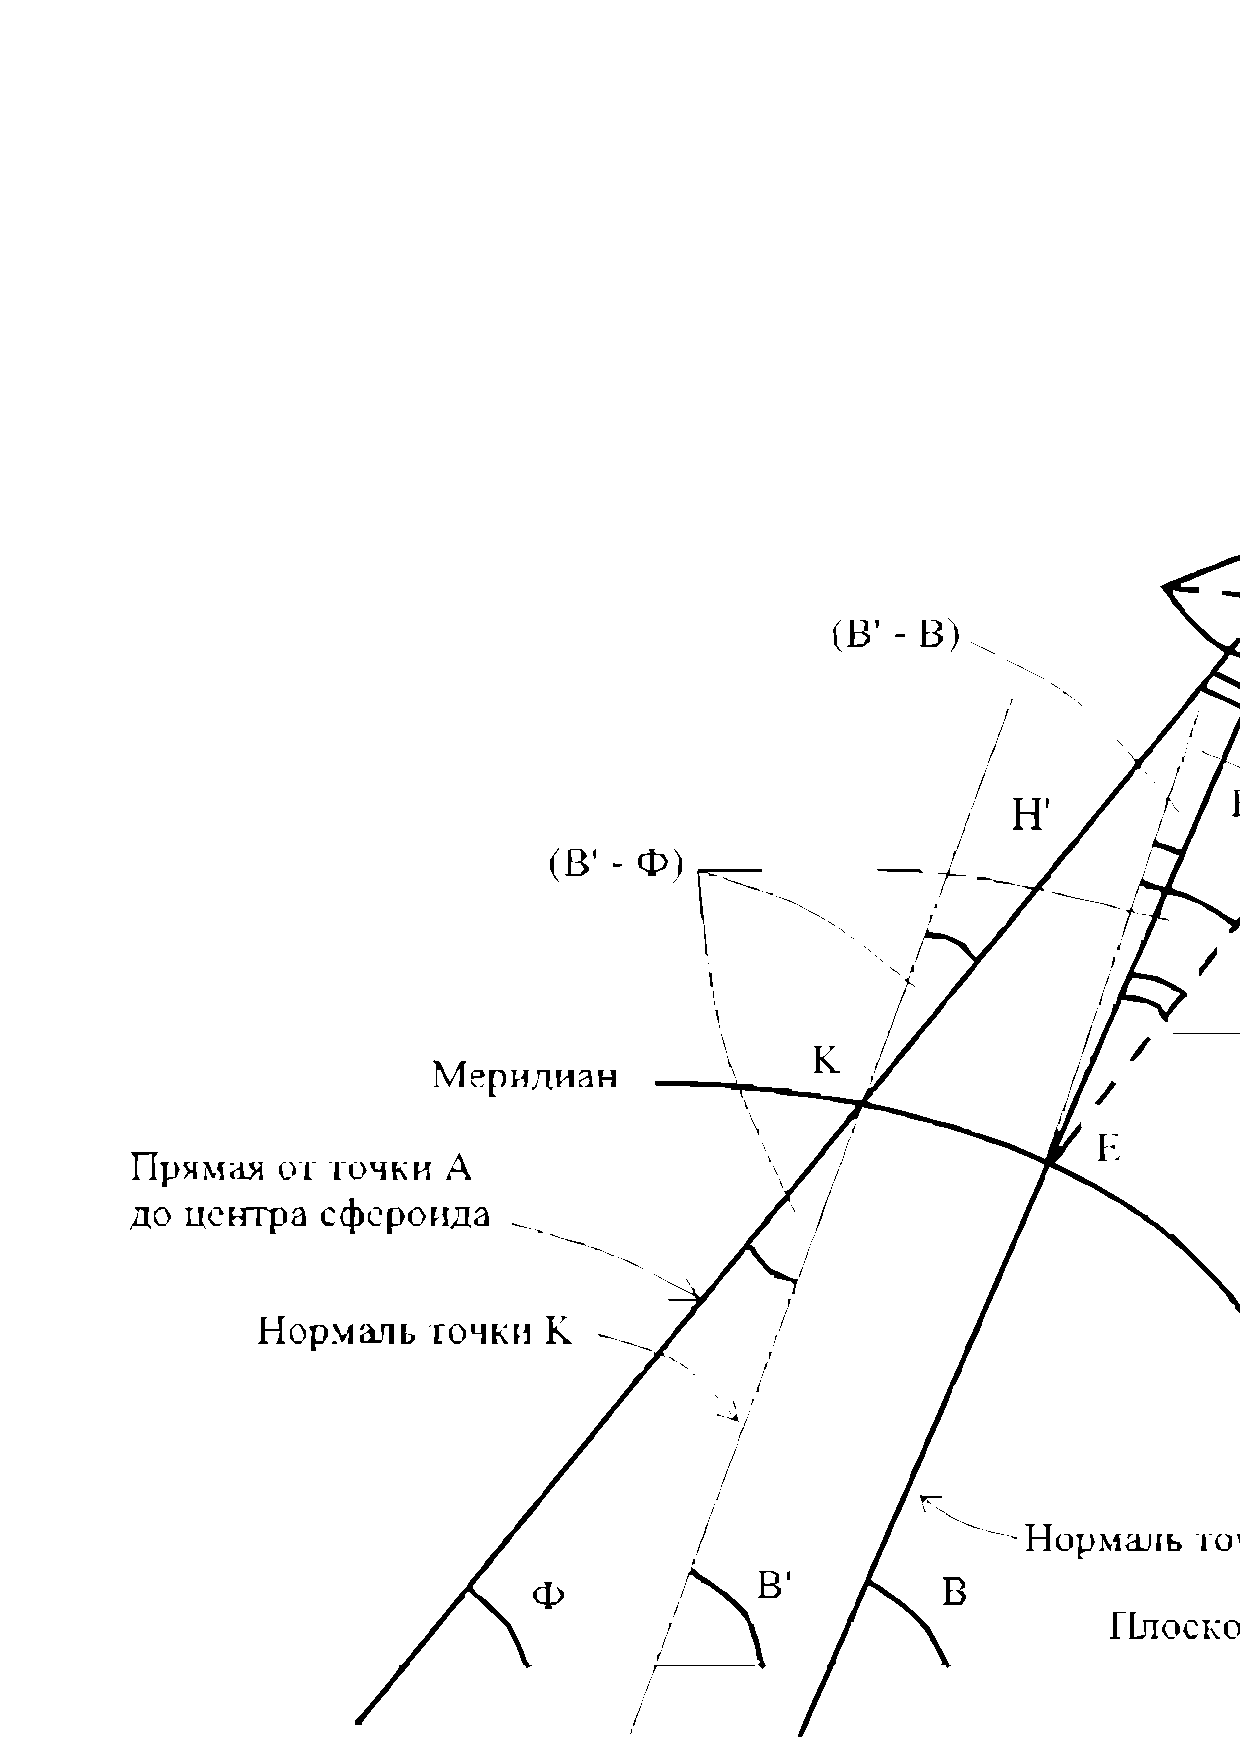
\includegraphics[scale=0.3]{ecef2geod}
\end{figure}
\note{
$\Phi$ -- геоцентрическая широта;
$B'$ -- геодезическая широта $K$;
$B$ -- геодезическая широта $A$
}
\end{frame}

\begin{frame}{Преобразование прямоугольных координат в геодезические}{Вспомогательные величины}
$$Q=\sqrt{X^2+Y^2+Z^2}$$
$$D=\sqrt{X^2+Y^2}$$
$$\Phi=\tan^{-1}\left(\frac{Z}{D}\right)$$
$$B'=\tan^{-1}\left(\frac{a^2}{b^2}\tan\Phi\right)$$
$$S=\frac{b}{\sqrt{1-e^2\cos^2\Phi}}$$
$$\Delta B=B'-\Phi$$

\note{
$S$ -- полудиаметр меридианного эллипса, продолжение которого проходит через точку $А$
}
\end{frame}

\begin{frame}{Преобразование прямоугольных координат в геодезические}
$$L=\tan^{-1}\left(\frac{Y}{X}\right)$$
$$B=B'-\frac{(Q-S)\Delta B\cos\Delta B}{S}$$
$$H=(Q-S)\cos\Delta B$$

\note{
$L$ -- геодезическая долгота;
$B$ -- геодезическая широта;
$H$ -- геодезическая высота
}
\end{frame}

\begin{frame}{Преобразование прямоугольных координат}{Параметры преобразования}
\begin{itemize}
\item $\Delta X$, $\Delta Y$, $\Delta Z$ -- вектор смещения
\item $\omega_x$, $\omega_y$, $\omega_z$ -- повороты
\item $m$ -- масштабирование в миллионных частях
\end{itemize}
\note{
Для преобразование прямоугольных координат используется преобразование Гельмерта. Для него необходимо знать 7 параметров: 3 смещения, 3 поворота и масштабный параметр.
}
\end{frame}

\begin{frame}{Формула преобразования прямоугольных координат}
 $$\begin{pmatrix} X\\Y\\Z \end{pmatrix}_b
 =(1+m)
\begin{pmatrix}
1 & \omega_z & -\omega_y\\
-\omega_z & 1 & \omega_x\\
\omega_y & -\omega_x & 1
\end{pmatrix}
\begin{pmatrix} X\\Y\\Z \end{pmatrix}_a +\begin{pmatrix}\Delta X\\\Delta Y\\\Delta Z\end{pmatrix}
$$
\end{frame}

\begin{frame}{Проекция Гаусса-Крюгера}
\begin{figure}
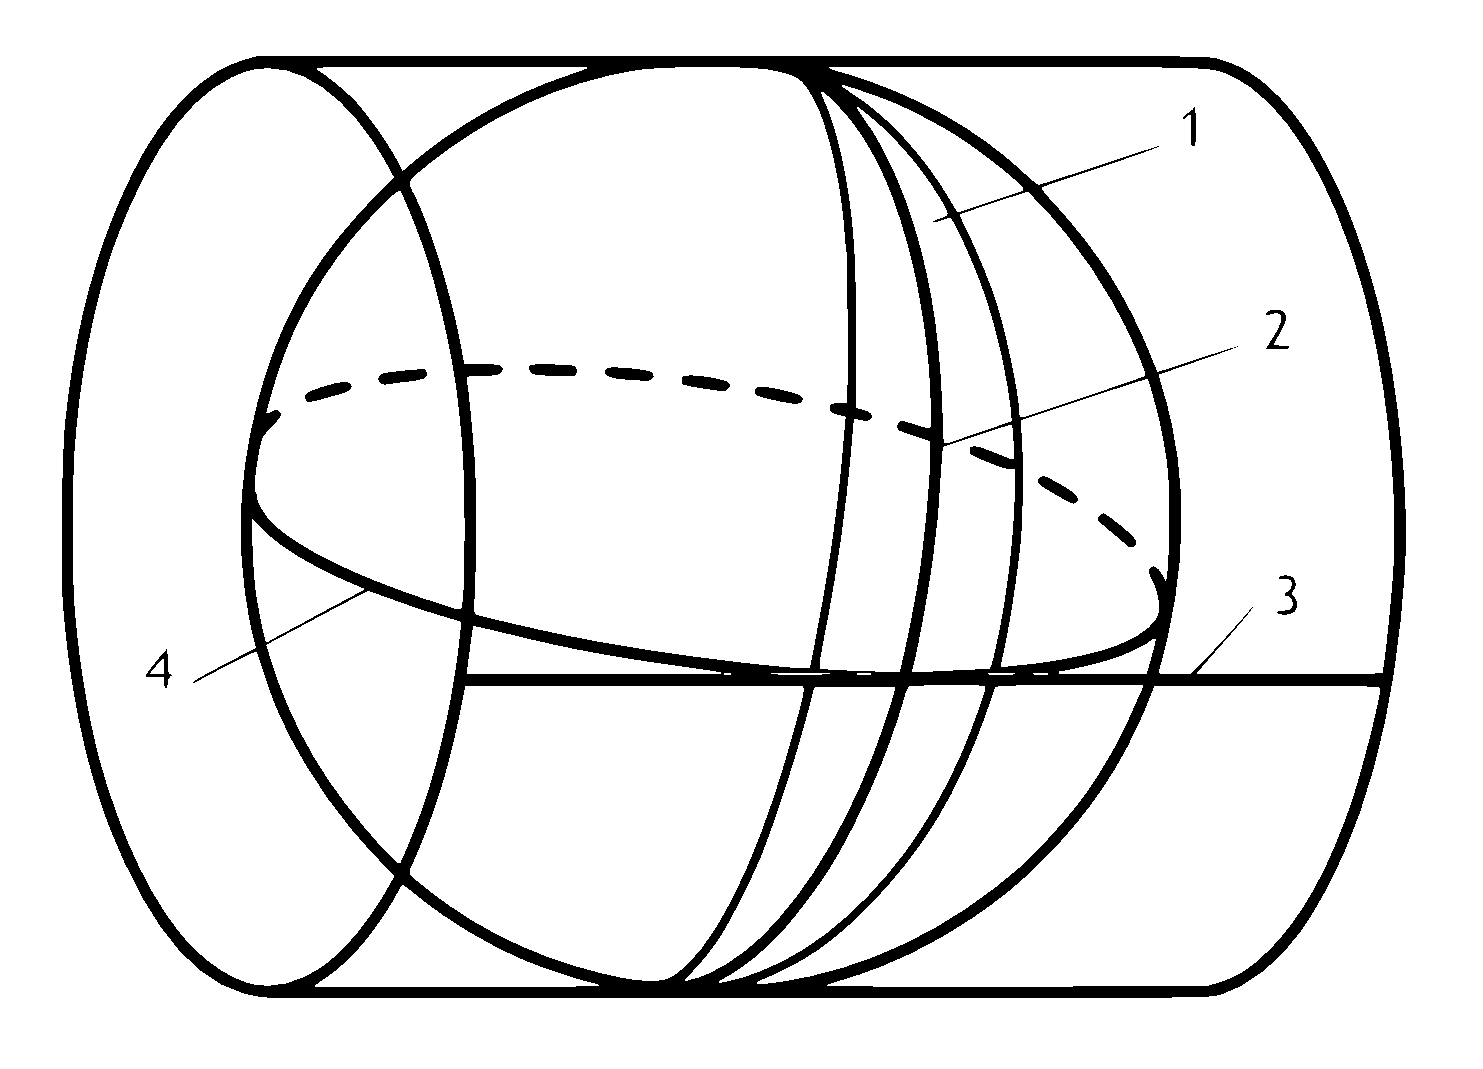
\includegraphics[scale=0.35]{tmerc}
\end{figure}
\note{
Проекция Гаусса-Крюгера - поперечная цилиндрическая равноугольная проекция. Расстояния являются точными вдоль центрального меридиана, если масштабный коэффициент равен 1,0. Если он меньше 1.0, точный масштаб сохраняется на двух приблизительно прямых линиях (при использовании эллипсоида), расположенных на равных расстояниях по обе стороны от центрального меридиана.

1 - зона, 2 - осевой (средний) меридиан зоны, 3 - проекция экватора на поверхность цилиндра, 4 - экватор
}
\end{frame}

%\subsection{Задание}
\begin{frame}{Преобразование геодезических координат в плоские прямоугольные}{Параметры проекции Гаусса-Крюгера}
\begin{itemize}
\item $B_0$ - широта центра проекции
\item $L_0$ - долгота центра проекции
\item $k_0$ - масштаб на центральном меридиане
\item $X_0$ - сдвиг по оси абсцисс
\item $Y_0$ - сдвиг по оси ординат
\end{itemize}
\note{
Для перевода геодезических координат в плоские прямоугольные проекции Гаусса-Крюгера используются 5 параметров.
\begin{itemize}
\item $B_0$ - широта центра проекции
\item $L_0$ - долгота центра проекции
\item $k_0$ - масштаб на центральном меридиане
\item $X_0$ - сдвиг по оси абсцисс
\item $Y_0$ - сдвиг по оси ординат
\end{itemize}
}
\end{frame}

\begin{frame}{Преобразование геодезических координат в плоские прямоугольные}{Проекция Гаусса-Крюгера}
\begin{multline}\nonumber
x = 6367558.4968 B -\\- \sin 2B (16002.8900 + 66.9607 \sin2 B + 0.3515 \sin4 B -\\
-l^2 (1594561.25 + 5336.535 \sin2 B + 26.790 \sin4 B + 0.149 \sin6 B +\\
+ l^2 (672483.4 - 811219.9 \sin2 B + 5420.0 \sin4 B - 10.6 \sin6 B +\\
+ l^2 (278194 - 830174 \sin2 B + 572434 \sin4 B - 16010 \sin6 B +\\
+ l^2 (109500 - 574700 \sin2 B + 863700 \sin4 B - 398600 \sin6 B)))))
\end{multline}
\note{
Вот формула для одной координаты из ГОСТ 51794-2008, здесь $B$ -- геодезическая широта, параметры $l$ и $n$ будут объяснены немного позже.
}
\end{frame}

\begin{frame}{Преобразование геодезических координат в плоские прямоугольные}{Проекция Гаусса-Крюгера}
\begin{multline}\nonumber
y = (5 + 10 n)  105 +\\+ l \cos B (6378245 + 21346.1415 \sin2 B +107.1590 \sin4 B +\\
+ 0.5977 \sin6 B +\\+ l^2 (1070204.16 - 2136826.66 \sin2 B + 17.98 \sin4 B - 11.99 \sin6 B +\\
+ l^2 (270806 - 1523417 \sin2 B + 1327645 \sin4 B - 21701 \sin6 B +\\
+ l^2 (79690 - 866190 \sin2 B + 1730360 \sin4 B - 945460 \sin6 B))))
\end{multline}
\note{
Вот формула для второй координаты из ГОСТа
}
\end{frame}

\begin{frame}{Преобразование геодезических координат в плоские прямоугольные}{Проекция Гаусса-Крюгера}
$$l=\{L-[3+6(n-1)]\}/57.29577951$$
$$n=\lfloor(6+L)/6\rfloor$$
\note{
$l$ -- расстояние от определяемой точки до осевого меридиана зоны в радианной мере.

$n$ -- номер шестиградусной зоны
}
\end{frame}

\begin{frame}{Менее ``страшные'' формулы}{Вспомогательные коэффициенты}
$$c=\cos B\mbox{, }s=\sin B$$
$$\nu=a\sqrt{\frac{1+\varepsilon}{1+\varepsilon c^2}}$$
$$\varepsilon=\frac{a^2-b^2}{b^2}\mbox{, }n=\frac{a-b}{a+b}$$
$$A=\frac{a}{1+n}\left(1+\frac{n^2}{8}\right)^2\mbox{, }B_1=1-\frac{3}{8}n^2$$
\begin{multline}\nonumber
m=A \bigg(B-B_1\bigg(\frac{3}{2}n\sin2B-\frac{15}{16}n^2\sin4B+\\+\frac{35}{48}n^3\sin6B-\frac{315}{512}n^4\sin8B\bigg)\bigg)
\end{multline}
\note{
Есть и другой вариант формул для перехода к проекции, здесь представлены вспомогательные коэффициенты.
}
\end{frame}

\begin{frame}
$$z=\frac{\varepsilon\omega^3c^5}{6}\mbox{, }\tan\theta_2=\frac{2sc\sin^2\left(\frac{\omega}{2}\right)}{s^2+c^2\cos\omega}$$
$$Y=k_0\left(m+\nu\theta_2+\frac{z\nu\omega s}{4}\left(9+4\varepsilon c^2-11\omega^2+20\omega^2c^2\right)\right)+Y_0$$
$$X=k_0\nu\left(\tanh^{-1}\left(c\sin\omega\right)+z\left(1+\frac{\omega^2}{10}\left(36c^2-29\right)\right)\right)+X_0$$
\note{
А здесь оставшиеся коэффициенты и формулы для координат в проекции Гаусса-Крюгера.
}
\end{frame}

\begin{frame}
\center Задание
\note{
Ну и теперь вам предстоит задание по переводу геодезических координат WGS84 в координаты в проекции Гаусса-Крюгера.
}
\end{frame}

\begin{frame}{Алгоритм}
\begin{enumerate}
\item Перейти от $B$, $L$, $H$ WGS84 к $X$, $Y$, $Z$
\item Перейти от WGS84 к СК 1942
\item Перейти от $X$, $Y$, $Z$ СК 1942 к $B$, $L$, $H$
\item Перейти к проекции Гаусса-Крюгера
\end{enumerate}
\end{frame}

\begin{frame}{Что ожидается в качестве ответа}
\begin{enumerate}
\item Исходные данные: широта/долгота в градусах, высота в метрах
\item Прямоугольные координаты WGS84 в метрах
\item Прямоугольные координаты СК 1942 в метрах
\item Геодезические координаты СК 1942: широта/долгота в градусах, высота в метрах
\item Плоские прямоугольные координаты МСК1964
\end{enumerate}
\end{frame}

\begin{frame}{Параметры}{WGS84}
$$a=6378137\mbox{ м}$$
$$\alpha=1/298.257223563$$
\end{frame}

\begin{frame}{Параметры}{Эллипсоид Красовского}
$$a=6378245\mbox{ м}$$
$$\alpha=1/298.3$$
$$b=6356863.019\mbox{ м}$$
\end{frame}

\begin{frame}{Параметры}{Переход из WGS84 в СК 1942}
$$\Delta X=-23.57\mbox{ м}$$
$$\Delta Y=140.95\mbox{ м}$$
$$\Delta Z=79.8\mbox{ м}$$
$$\omega_x=0''$$
$$\omega_y=0.35''$$
$$\omega_z=0.79''$$
$$m=0.22\cdot10^{-6}$$
\end{frame}

\begin{frame}{Параметры}{Проекция для МСК1964}
$$L_0=30\degree$$
$$B_0=0\degree$$
$$k_0=1$$
$$X_0=95942.17\mbox{ м}$$
$$Y_0=-6552810\mbox{ м}$$
\end{frame}

\begin{frame}{Дополнительная литература}
\center\url{{https://goo.su/gost32453}}
\end{frame}

\begin{frame}
\center\url{{https://vk.com/movsesyanpv}}\\
\url{{https://t.me/movsesyanpv}}\\
\href{mailto:movsesyanpv@gmail.com}{movsesyanpv@gmail.com}\\
%\url{{https://astrotest.happyv0dka.cloud}}
\end{frame}
\end{document}


